\documentclass[a4paper,landscape]{article}
\usepackage[a4paper,landscape,margin=0.55cm]{geometry}
\usepackage{fontspec}
\usepackage{amsmath}
\usepackage{unicode-math}
\setmainfont{texgyreheros}[Extension=.otf,UprightFont=*-regular,BoldFont=*-bold,ItalicFont=*-italic,BoldItalicFont=*-bolditalic]
\setmathfont{texgyrepagella-math.otf}
\usepackage[table]{xcolor}
\usepackage{tikz}
\usetikzlibrary{arrows.meta,positioning,calc}
\usepackage{adjustbox}
\pagestyle{empty}

\definecolor{ink}{HTML}{14213D}
\definecolor{trust}{HTML}{2F7A4F}
\definecolor{curious}{HTML}{C8611E}
\definecolor{untrusted}{HTML}{A23B3B}
\definecolor{chan}{HTML}{2F5F98}
\definecolor{soft}{HTML}{F3EFE6}
\definecolor{softblue}{HTML}{E6EEF8}
\definecolor{softgreen}{HTML}{E4F1E8}
\definecolor{softred}{HTML}{F6E3E1}
\definecolor{grey}{HTML}{6B7280}
\definecolor{bankc}{HTML}{1F6F8B}
\definecolor{keyc}{HTML}{8E2C6E}

\newcommand{\bk}{\tikz[baseline=(c.base)]\node[fill=bankc,text=white,rounded corners=1pt,inner sep=1.2pt,font=\bfseries\fontsize{5.6}{6}\selectfont] (c) {bank};}
\newcommand{\ek}{\tikz[baseline=(c.base)]\node[fill=keyc,text=white,rounded corners=1pt,inner sep=1.2pt,font=\bfseries\fontsize{5.6}{6}\selectfont] (c) {enclave key};}
\newcommand{\num}[1]{\tikz[baseline=(c.base)]\node[circle,fill=ink,text=white,inner sep=0.8pt,font=\bfseries\fontsize{6}{6}\selectfont] (c) {#1};}
\newcommand{\hd}[1]{{\bfseries #1}}
\newcommand{\sm}{\fontsize{7.6}{9.2}\selectfont}
\newcommand{\xs}{\fontsize{6.8}{8.3}\selectfont}

\tikzset{
  lane/.style={draw=grey!60,dashed,line width=0.6pt},
  head/.style={draw,rounded corners=3pt,line width=1.1pt,font=\sm\bfseries,minimum width=3.6cm,minimum height=0.75cm,align=center},
  note/.style={draw=grey,fill=white,rounded corners=2pt,align=left,inner sep=3pt,font=\xs},
  arr/.style={-{Stealth[length=5pt]},line width=0.9pt,ink},
  sarr/.style={-{Stealth[length=5pt]},line width=0.9pt,chan},
  msg/.style={font=\xs,fill=white,inner sep=1.2pt,align=center},
}

\begin{document}
\noindent
\begin{adjustbox}{max width=\linewidth,max totalheight=\textheight,center}
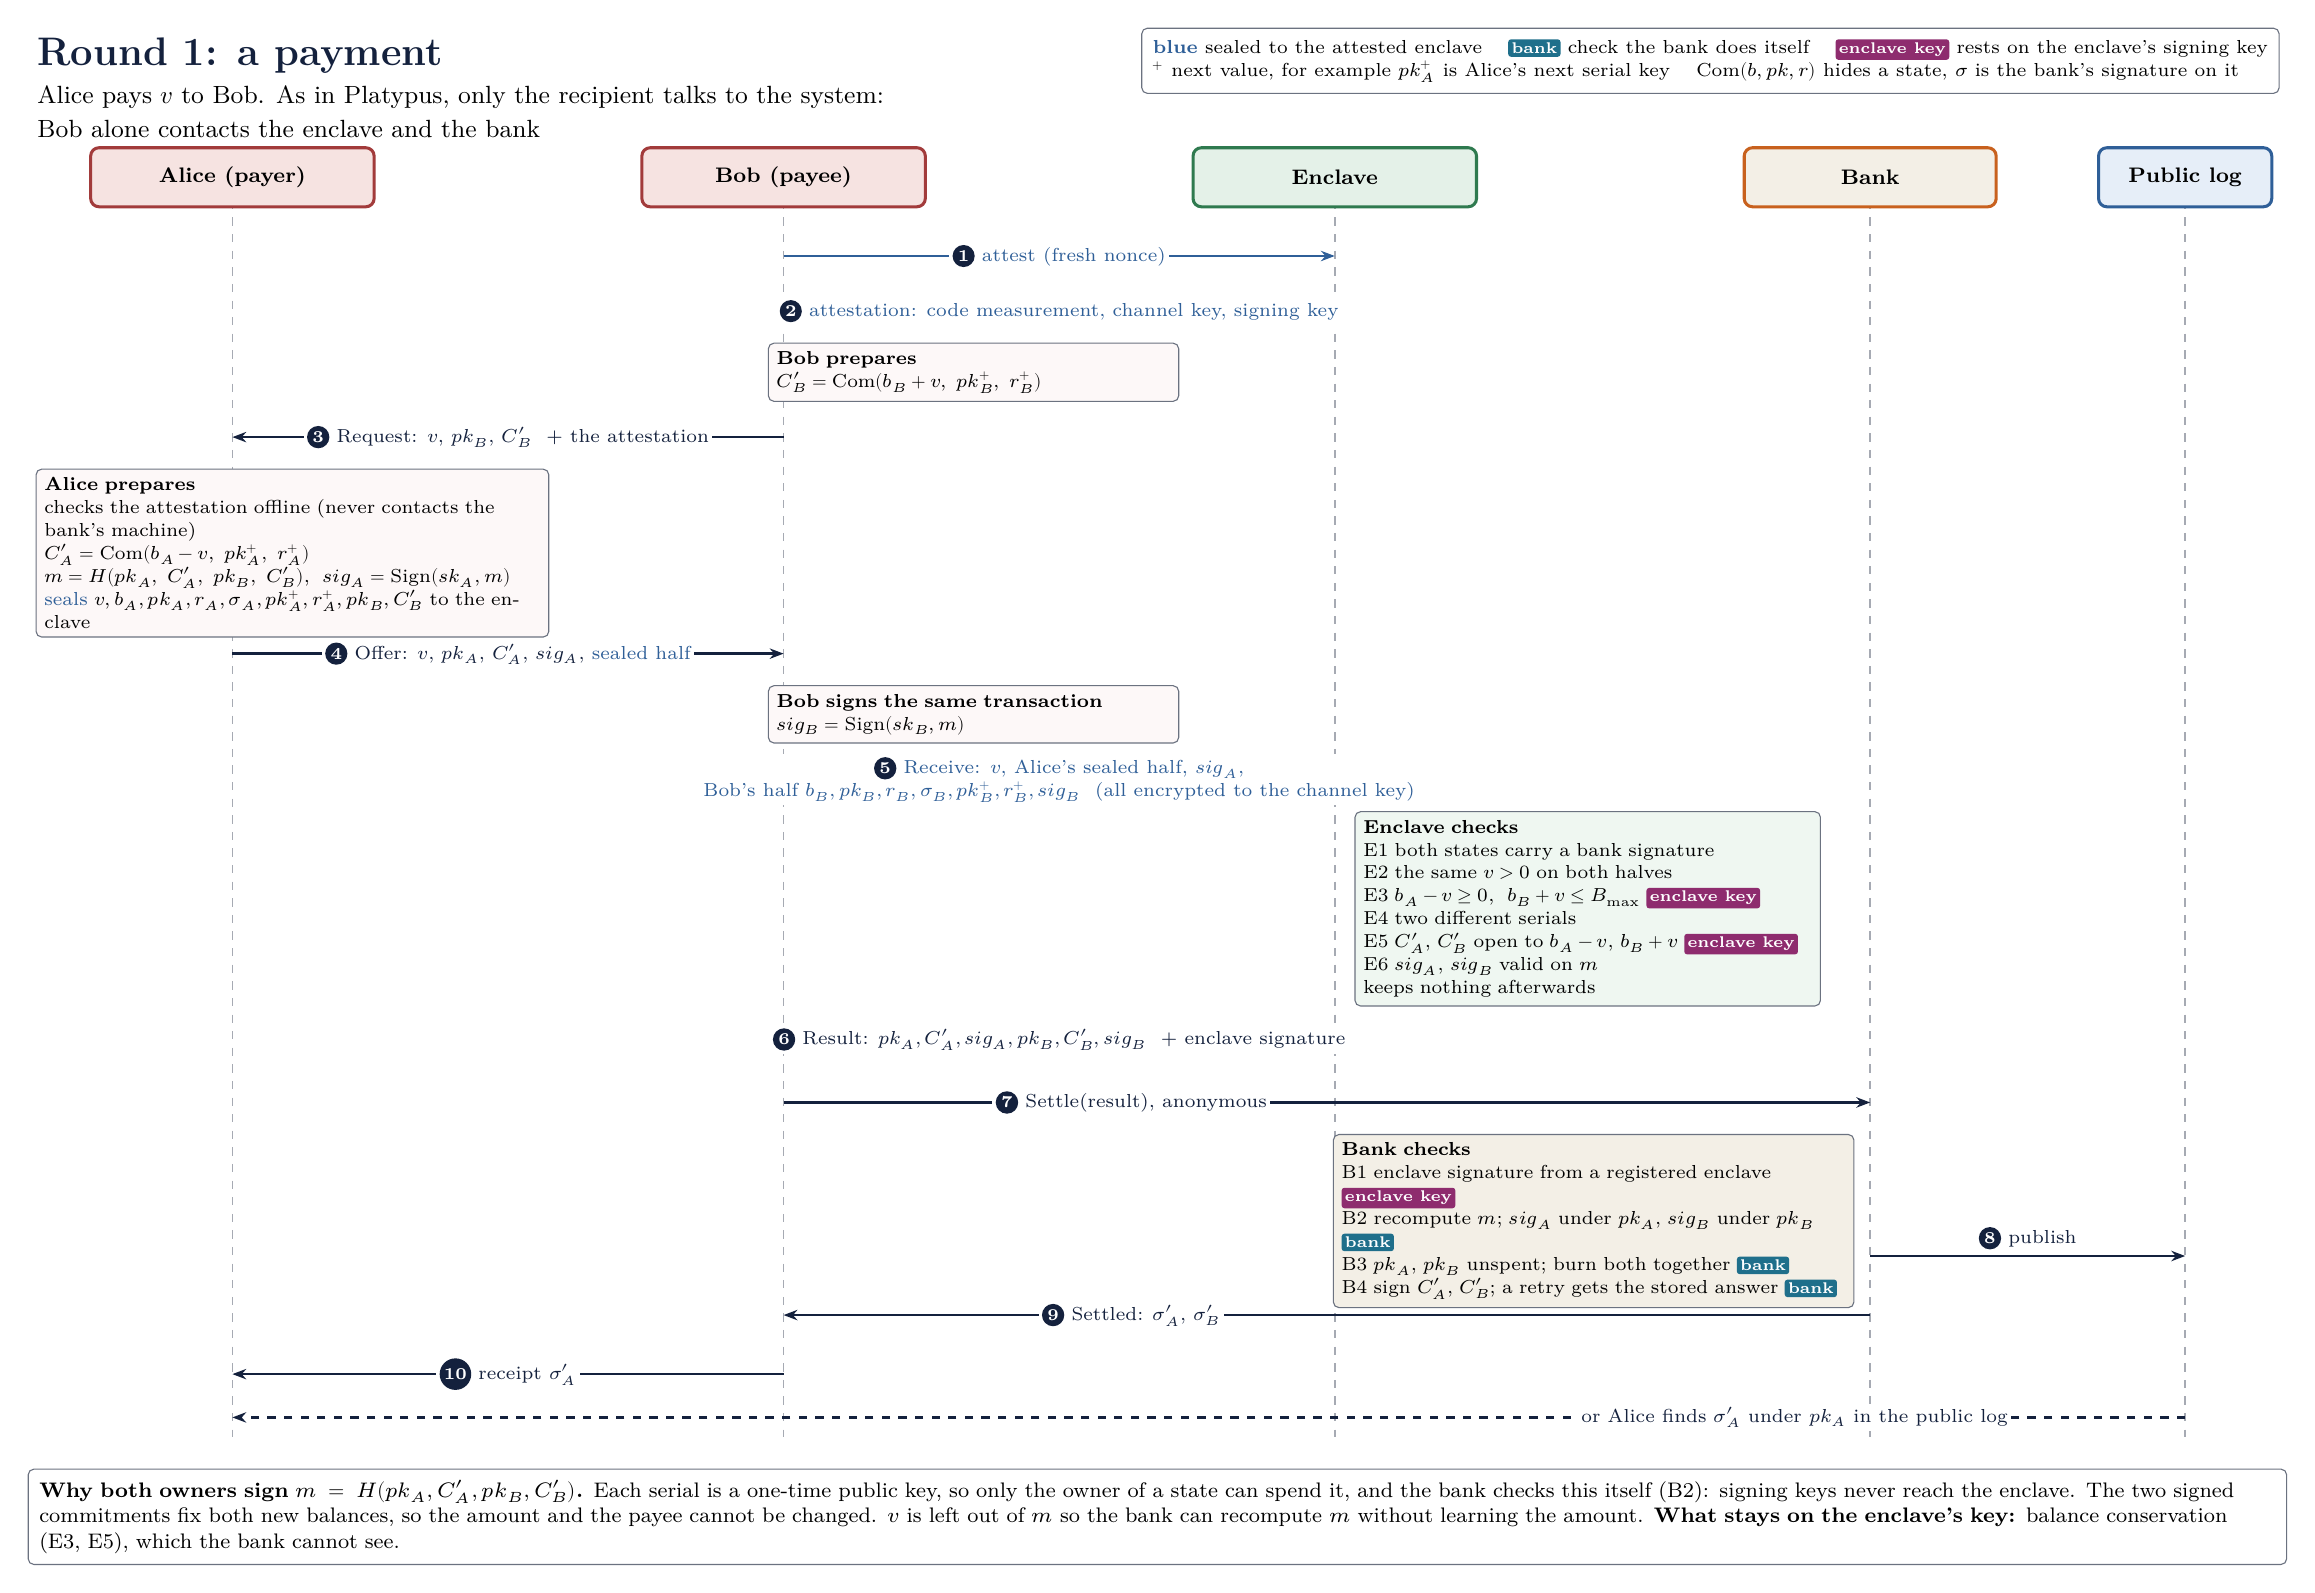
\begin{tikzpicture}[x=1cm,y=1cm]

\node[anchor=north west,align=left] at (0,20.2) {{\bfseries\Large\color{ink} Round 1: a payment}\\[2pt]{\small Alice pays $v$ to Bob. As in Platypus, only the recipient talks to the system:}\\{\small Bob alone contacts the enclave and the bank}};
\node[anchor=north east,align=left,font=\xs,draw=grey,rounded corners=2pt,inner sep=4pt] at (28.6,20.2) {
{\color{chan}\textbf{blue}} sealed to the attested enclave \quad \bk{} check the bank does itself \quad \ek{} rests on the enclave's signing key\\
$^{+}$ next value, for example $pk_A^{+}$ is Alice's next serial key \quad $\mathrm{Com}(b,pk,r)$ hides a state, $\sigma$ is the bank's signature on it};

\def\xa{2.6}\def\xb{9.6}\def\xe{16.6}\def\xk{23.4}\def\xl{27.4}
\foreach \x in {\xa,\xb,\xe,\xk,\xl} {\draw[lane] (\x,18.0) -- (\x,2.3);}
\node[head,draw=untrusted,fill=softred] at (\xa,18.3) {Alice (payer)};
\node[head,draw=untrusted,fill=softred] at (\xb,18.3) {Bob (payee)};
\node[head,draw=trust,fill=softgreen] at (\xe,18.3) {Enclave};
\node[head,draw=curious,fill=soft,minimum width=3.2cm] at (\xk,18.3) {Bank};
\node[head,draw=chan,fill=softblue,minimum width=2.2cm] at (\xl,18.3) {Public log};

\draw[sarr] (\xb,17.3) -- node[msg,text=chan]{\num{1} attest (fresh nonce)} (\xe,17.3);
\draw[sarr] (\xe,16.6) -- node[msg,text=chan]{\num{2} attestation: code measurement, channel key, signing key} (\xb,16.6);

\node[note,anchor=north west,text width=5.0cm,fill=softred!25] at (\xb-0.2,16.2) {\hd{Bob prepares}\\$C_B'=\mathrm{Com}(b_B+v,\ pk_B^{+},\ r_B^{+})$};
\draw[arr] (\xb,15.0) -- node[msg]{\num{3} Request: $v$, $pk_B$, $C_B'$ \ + the attestation} (\xa,15.0);

\node[note,anchor=north west,text width=6.3cm,fill=softred!25] at (0.1,14.6) {\hd{Alice prepares}\\
checks the attestation offline (never contacts the bank's machine)\\
$C_A'=\mathrm{Com}(b_A-v,\ pk_A^{+},\ r_A^{+})$\\
$m=H(pk_A,\ C_A',\ pk_B,\ C_B')$, \ $sig_A=\mathrm{Sign}(sk_A,m)$\\
{\color{chan}seals} $v, b_A, pk_A, r_A, \sigma_A, pk_A^{+}, r_A^{+}, pk_B, C_B'$ to the enclave};
\draw[arr] (\xa,12.25) -- node[msg]{\num{4} Offer: $v$, $pk_A$, $C_A'$, $sig_A$, {\color{chan}sealed half}} (\xb,12.25);

\node[note,anchor=north west,text width=5.0cm,fill=softred!25] at (\xb-0.2,11.85) {\hd{Bob signs the same transaction}\\$sig_B=\mathrm{Sign}(sk_B,m)$};
\draw[sarr] (\xb,10.65) -- node[msg,text=chan]{\num{5} Receive: $v$, {\color{chan}Alice's sealed half}, $sig_A$,\\Bob's half $b_B, pk_B, r_B, \sigma_B, pk_B^{+}, r_B^{+}, sig_B$ \ (all encrypted to the channel key)} (\xe,10.65);

\node[note,anchor=north west,text width=5.7cm,fill=softgreen!60] at (\xe+0.25,10.25) {\hd{Enclave checks}\\
E1 both states carry a bank signature\\
E2 the same $v>0$ on both halves\\
E3 $b_A-v\ge 0$, \ $b_B+v\le B_{\max}$ \ek{}\\
E4 two different serials\\
E5 $C_A'$, $C_B'$ open to $b_A-v$, $b_B+v$ \ek{}\\
E6 $sig_A$, $sig_B$ valid on $m$\\
keeps nothing afterwards};
\draw[arr] (\xe,7.35) -- node[msg]{\num{6} Result: $pk_A, C_A', sig_A, pk_B, C_B', sig_B$ \ + enclave signature} (\xb,7.35);

\draw[arr] (\xb,6.55) -- node[msg,pos=0.32]{\num{7} Settle(result), anonymous} (\xk,6.55);
\node[note,anchor=north east,text width=6.4cm,fill=soft] at (\xk-0.2,6.15) {\hd{Bank checks}\\
B1 enclave signature from a registered enclave \ek{}\\
B2 recompute $m$; $sig_A$ under $pk_A$, $sig_B$ under $pk_B$ \bk{}\\
B3 $pk_A$, $pk_B$ unspent; burn both together \bk{}\\
B4 sign $C_A'$, $C_B'$; a retry gets the stored answer \bk{}};
\draw[arr] (\xk,4.6) -- node[msg,above=1pt]{\num{8} publish} (\xl,4.6);
\draw[arr] (\xk,3.85) -- node[msg,pos=0.68]{\num{9} Settled: $\sigma_A'$, $\sigma_B'$} (\xb,3.85);
\draw[arr] (\xb,3.1) -- node[msg]{\num{10} receipt $\sigma_A'$} (\xa,3.1);
\draw[arr,dashed] (\xl,2.55) -- node[msg,pos=0.2]{or Alice finds $\sigma_A'$ under $pk_A$ in the public log} (\xa,2.55);

\node[anchor=north west,text width=28.4cm,align=left,font=\sm,draw=grey,rounded corners=2pt,inner sep=4pt] at (0,1.9) {
\hd{Why both owners sign $m=H(pk_A, C_A', pk_B, C_B')$.} Each serial is a one-time public key, so only the owner of a state can spend it, and the bank checks this itself (B2): signing keys never reach the enclave. The two signed commitments fix both new balances, so the amount and the payee cannot be changed. $v$ is left out of $m$ so the bank can recompute $m$ without learning the amount. \hd{What stays on the enclave's key:} balance conservation (E3, E5), which the bank cannot see.};

\end{tikzpicture}
\end{adjustbox}
\end{document}
